\chapter{Introduction}

After the Master's Degree at Telecom, I joined Alkemics team to tackle data-quality challenges involving predicting methods. 

Before diving in the machine-learning related challenges, this chapter will present Alkemics, its proposition value, and its technological stack.

\section{Alkemics}


Alkemics connects brands and retailers to help them market \& sell their products everywhere, driving business growth, by allowing them to collect, enrich, and share product data across the retail ecosystem.

Our mission is to connect every brand with every retailer in the world. The platform streamlines the management of digital product content (i.e., packaging, ingredients, visuals, promotions, rich media), extracts structured metadata for optimal quality and usability, and automates delivery to retail partners and third party service providers.

Founded in 2011, and backed by world renowned investors (Index Ventures, Serena Capital, Cathay Innovation, Partech Ventures, among others), Alkemics consists of more than 70 employees.


\subsection{Alkemics Plateform}

Because of increasing regulations, new customer demands, omni-channel communications, there is a growing need for richer and more exhaustive product information. 

Yet the difficulties to gather this data keep growing: the number of products is growing exponentially, some products identification numbers change more than 10 times per year (promotion, seasonality, new recipes, new packagings...), and overall, 40\% of products identification numbers are renewed every year.

This cascades in a series of problems that handicap manufacturers, retailers and consumers: logistics struggle to maintain stock, accounting systems fail to track how different products are actually the same consumption unit, pricing teams struggle to maintain price coherency in this dynamic environment, marketing teams are inefficient to share richer and richer content about the product, BI teams feel that the consumption of the consumer are changing while they actually don't. 

Alkemics solution to these challenges is a plateform that enables:
\\

\textbf{Makers} to:
    \begin{itemize}
    \item Collect product information from all the stakeholders of the organization: the \textit{supply team} who knows the size and weight of the product, the \textit{marketing team} who owns the pictures, videos as well as the brand content, the \textit{quality team} who masters the composition, nutritional values, etc.
    \item Store product information in a centralized way, so everyone in the organization can have access to it.
    \item Distribute product information so every partner has the same up-to-date information. This includes retailers, but also marketing agencies, trade marketing agencies, ...
    \item Collaborate with 3rd parties to collect user reviews,  receive data quality reports,  print coupons, use buy-it-now solutions.
    \end{itemize}

\textbf{Retailers} to:
    \begin{itemize}
    \item Have access to best-in-class product information to power their tools and feed their digital supports 
    \item Collaborate with manufacturers to reference new products \& innovations, run call-for-proposals for promotional formats, etc…
    \item Connect products that share a given set of attributes in order to understand how they relate
    \end{itemize}

\begin{figure}[H]
\centering
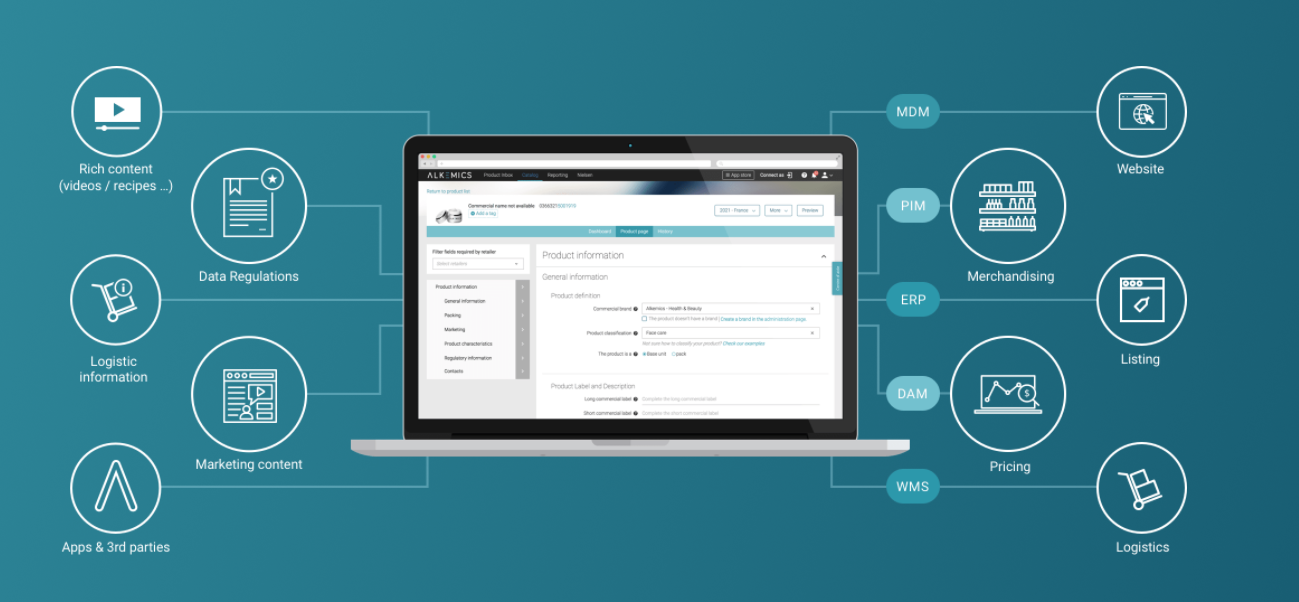
\includegraphics[scale=0.35]{./images/alkemics_website_global.png}
\caption{Alkemics plateform}
\end{figure}


\subsection{The technological stack}

\textbf{Micro-services architecture}
The stack in Alkemics is composed of set of dozens of micro services communicating with synchronous calls (HTTPS) and both synchronous and asynchronous messaging (TCP enabled by Rabbit MQ).
Each service has a domain specific task: data ingestion, data classification, APIs for merchandising, etc. A subset of the services are exposed to third parties and clients.

\textbf{User interface}
User Interface dashboards also call the APIs to make functionalities available to the users (makers and retailers) trough a web browser.
The front part of the website is implemented with React framework.

\textbf{APIs and SDKs}
A set of SDKs are also provided to retailers to allow them to use merchandising functionalities directly embedded in their websites.

\textbf{Storage vs indexation}
All Alkemics crucial data is stored in relational databases (MySQL). Yet if relationnal databases provide very useful functionalities to guaranty integrity of data, its indexing capabilities remain quite poor in comparison to non-relational databases.

That's we also create ElasticSearch indexes, containing data that is already stored in relational databases, but indexed in a format allowing quick and performant queries.


\section{Professional thesis objective}

This professional thesis aims at implementing machine learning techniques to improve products data quality.
